\documentclass{standalone}

\usepackage{tikz}
\usetikzlibrary{arrows}
\usetikzlibrary{decorations.markings}
\usepackage{standalone}

\begin{document}

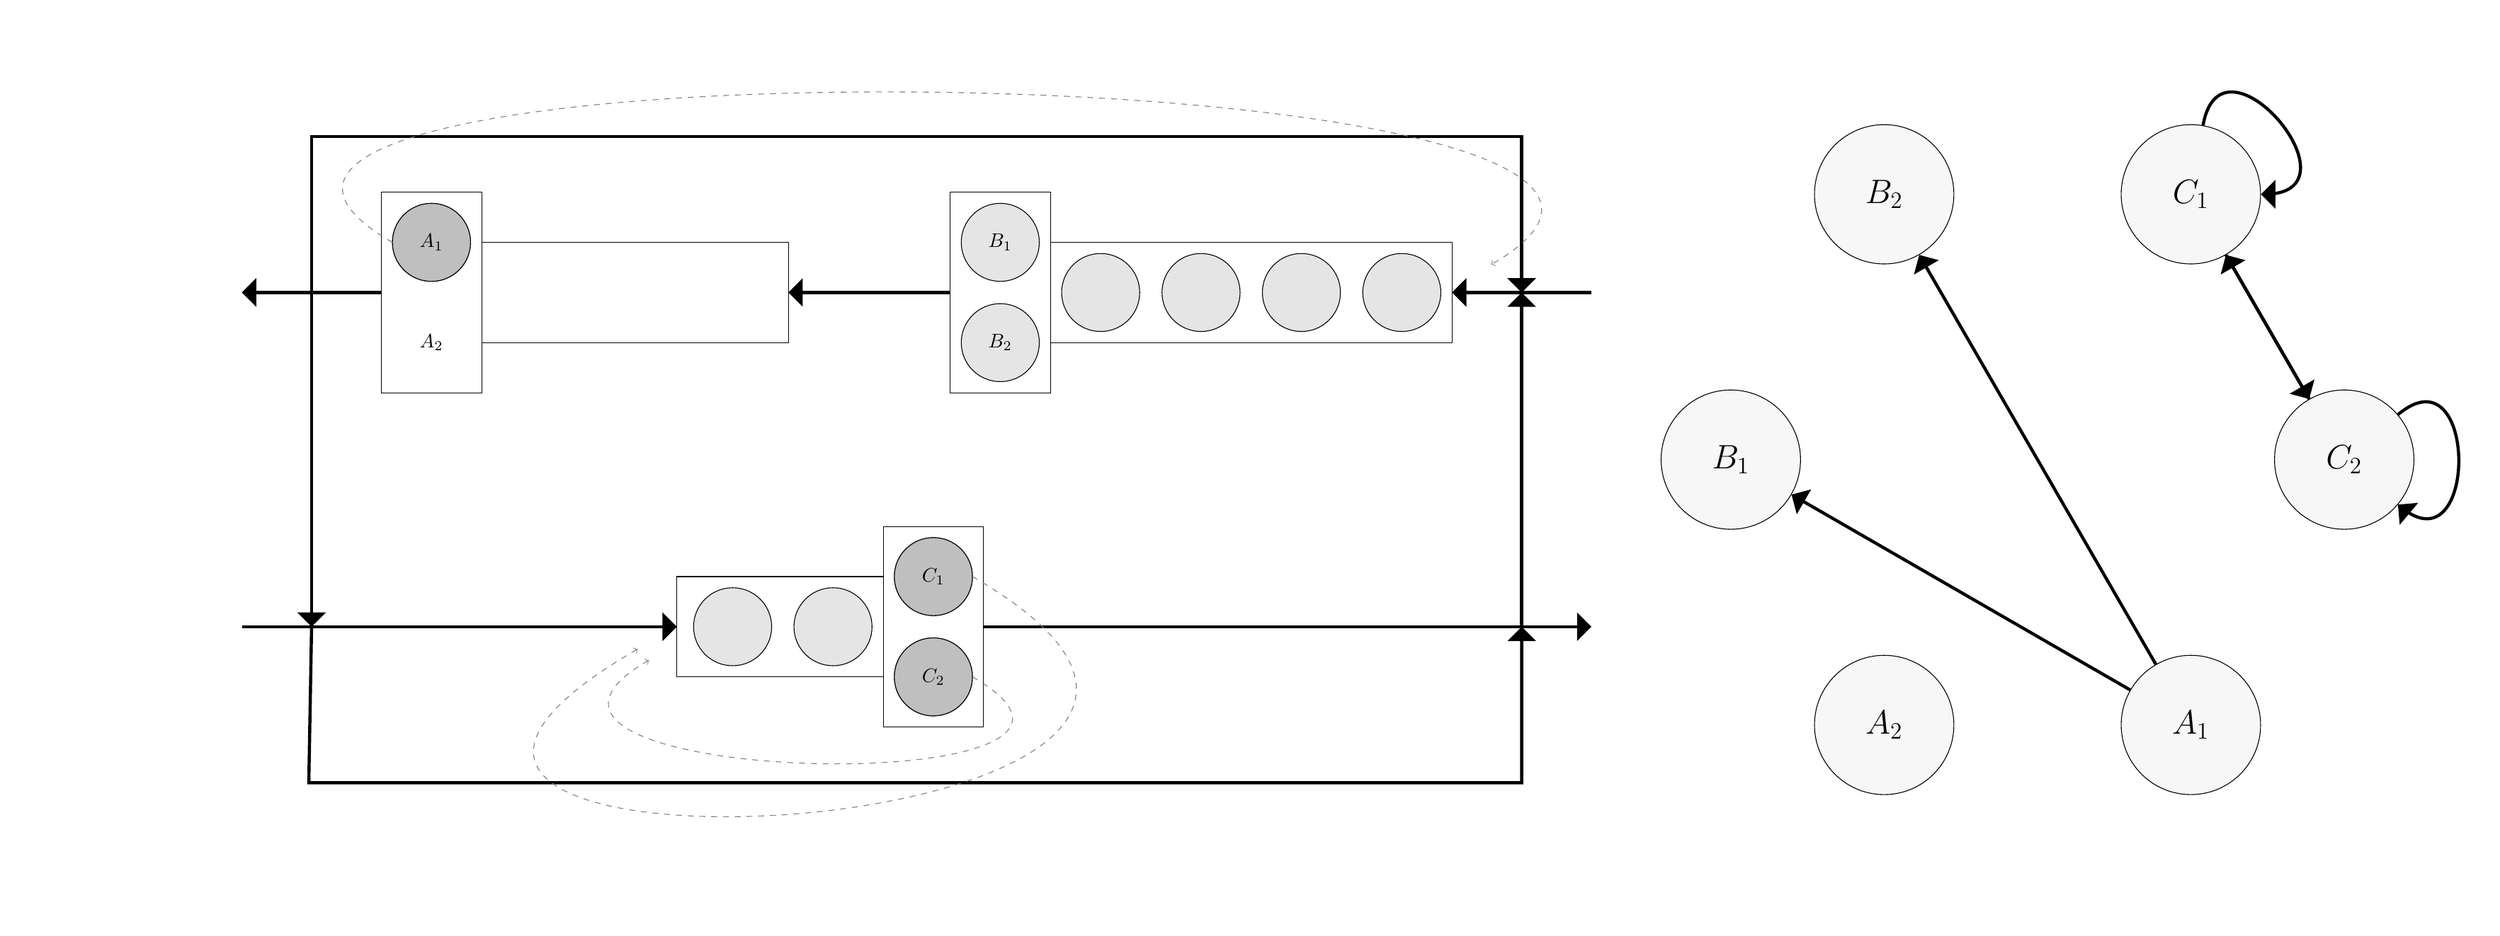
\begin{tikzpicture}

% Node bottom
\draw (-1.9, 2.1) rectangle (1.8, 3.9);
\draw (1.8, 1.2) rectangle (3.6, 4.8);

% Nodes middle
\draw (4.8, 8.1) rectangle (12, 9.9);
\draw (3, 7.2) rectangle (4.8, 10.8);

\draw (-5.4, 8.1) rectangle (0.1, 9.9);
\draw (-7.2, 7.2) rectangle (-5.4, 10.8);

% Routings
\draw[ultra thick, -triangle 90] (14.5, 9) -- (12, 9); % in to middle
\draw[ultra thick, -triangle 90] (3, 9) -- (0.1, 9); % middle to middle
\draw[ultra thick, -triangle 90] (-7.2, 9) -- (-9.7, 9); % out of middle

\draw[ultra thick, -triangle 90] (-9.7, 3) -- (-1.9, 3); % In to bottom
\draw[ultra thick, -triangle 90] (3.6, 3) -- (14.5, 3); % Out of bottom

\draw[ultra thick, -triangle 90] (-8.45, 9) -- (-8.45, 3); % middle to bottom
\draw[ultra thick, -triangle 90] (13.25, 3) -- (13.25, 9); % bottom to middle

\draw[ultra thick, -triangle 90] (-8.45, 9) -- (-8.45, 11.8) -- (13.25, 11.8) -- (13.25, 9); % top left to top right
\draw[ultra thick, -triangle 90] (-8.45, 3) -- (-8.5, 0.2) -- (13.25, 0.2) -- (13.25, 3); % bottom loop

% middle left
\node[align=center] [style={minimum size=1.4cm, text width=1.0cm, draw=black,fill=black!10,text=black,shape=circle}] at (-6.3, 9.9) {$A_1$};
% \node[align=center] [style={minimum size=1.4cm, text width=1.0cm, draw=black,fill=black!10,text=black,shape=circle}] at (-6.3, 8.1) {$A_2$};
\node[align=center] [style={minimum size=1.4cm, text width=1.0cm, draw=none,fill=none,shape=circle}] at (-6.3, 8.1) {$A_2$};
% \node[align=center] [style={minimum size=1.4cm, text width=1.0cm, draw=black,fill=black!10,text=black,shape=circle}] at (-4.5, 9) {};
% \node[align=center] [style={minimum size=1.4cm, text width=1.0cm, draw=black,fill=black!10,text=black,shape=circle}] at (-2.7, 9) {};
% \node[align=center] [style={minimum size=1.4cm, text width=1.0cm, draw=black,fill=black!10,text=black,shape=circle}] at (-0.9, 9) {};

% middle right
\node[align=center] [style={minimum size=1.4cm, text width=1.0cm, draw=black,fill=black!10,text=black,shape=circle}] at (3.9, 9.9) {$B_1$};
\node[align=center] [style={minimum size=1.4cm, text width=1.0cm, draw=black,fill=black!10,text=black,shape=circle}] at (3.9, 8.1) {$B_2$};
\node[align=center] [style={minimum size=1.4cm, text width=1.0cm, draw=black,fill=black!10,text=black,shape=circle}] at (5.7, 9) {};
\node[align=center] [style={minimum size=1.4cm, text width=1.0cm, draw=black,fill=black!10,text=black,shape=circle}] at (7.5, 9) {};
\node[align=center] [style={minimum size=1.4cm, text width=1.0cm, draw=black,fill=black!10,text=black,shape=circle}] at (9.3, 9) {};
\node[align=center] [style={minimum size=1.4cm, text width=1.0cm, draw=black,fill=black!10,text=black,shape=circle}] at (11.1, 9) {};

% Bottom customers
\node[align=center] [style={minimum size=1.4cm, text width=1.0cm, draw=black,fill=black!10,text=black,shape=circle}] at (10.2-7.5, 3.9) {$C_1$};
\node[align=center] [style={minimum size=1.4cm, text width=1.0cm, draw=black,fill=black!10,text=black,shape=circle}] at (10.2-7.5, 2.1) {$C_2$};
\node[align=center] [style={minimum size=1.4cm, text width=1.0cm, draw=black,fill=black!10,text=black,shape=circle}] at (6.6-7.5, 3) {};
\node[align=center] [style={minimum size=1.4cm, text width=1.0cm, draw=black,fill=black!10,text=black,shape=circle}] at (8.4-7.5, 3) {};

% State digraph Nodes


\node (A1) [style={minimum size=2.5cm,draw=black,fill=black!3,text=black,shape=circle}] at (25.25, 1.237) {\LARGE{$A_1$}};
\node (A2) [style={minimum size=2.5cm,draw=black,fill=black!3,text=black,shape=circle}] at (19.75, 1.237) {\LARGE{$A_2$}};
\node (B1) [style={minimum size=2.5cm,draw=black,fill=black!3,text=black,shape=circle}] at (17, 6) {\LARGE{$B_1$}};
\node (B2) [style={minimum size=2.5cm,draw=black,fill=black!3,text=black,shape=circle}] at (19.75, 10.763) {\LARGE{$B_2$}};
\node (C1) [style={minimum size=2.5cm,draw=black,fill=black!3,text=black,shape=circle}] at (25.25, 10.763) {\LARGE{$C_1$}};
\node (C2) [style={minimum size=2.5cm,draw=black,fill=black!3,text=black,shape=circle}] at (28, 6) {\LARGE{$C_2$}};

% A1 to B
\node[align=center] [style={minimum size=1.4cm, text width=1.0cm, draw=black,fill=black!25,text=black,shape=circle}] at (-6.3, 9.9) {$A_1$};
\draw[ultra thick, -triangle 90] (A1) -- (B1);
\draw[ultra thick, -triangle 90] (A1) -- (B2);
\draw[gray, dashed, ->] (-7, 9.9) [out=150, in=30, looseness=1] to (12.7, 9.5);

% C1 to C
\node[align=center] [style={minimum size=1.4cm, text width=1.0cm, draw=black,fill=black!25,text=black,shape=circle}] at (10.2-7.5, 2.1) {$C_2$};
\draw[ultra thick, -triangle 90] (C2) -- (C1);
\draw[ultra thick, -triangle 90] (C2) [out=40, in=-40, looseness=3] to (C2);
\draw[gray, dashed, ->] (10.9-7.5, 2.1) [out=-30, in=-150, looseness=2] to (-2.4, 2.4);

% C1 to C
\node[align=center] [style={minimum size=1.4cm, text width=1.0cm, draw=black,fill=black!25,text=black,shape=circle}] at (10.2-7.5, 3.9) {$C_1$};
\draw[ultra thick, -triangle 90] (C1) [out=80, in=0, looseness=3] to  (C1);
\draw[ultra thick, -triangle 90] (C1) -- (C2);
\draw[gray, dashed, ->] (10.9-7.5, 3.9) [out=-30, in=-150, looseness=4] to (-2.6, 2.6);


\end{tikzpicture}

\end{document}
